\documentclass[a0,portrait]{a0poster}

\usepackage{multicol}
\columnsep=100pt
\columnseprule=3pt

\usepackage{times}
\usepackage{graphicx}
\graphicspath{{../}}
\usepackage{booktabs}
\usepackage[font=small,labelfont=bf]{caption}
\usepackage{amsfonts, amsmath, amsthm, amssymb, marvosym}
\usepackage{wrapfig}
\usepackage{enumitem}
\usepackage{fancyvrb}
\usepackage{xspace}
\usepackage[svgnames,usenames,dvipsnames]{xcolor}

%\usepackage{algorithm}
%\usepackage[noend]{algorithmic}
\usepackage{algpseudocode}

\def\texttts#1{\texttt{\large#1}}

\begin{document}

%---------------------------------------------------------------
%	POSTER HEADER 
%---------------------------------------------------------------
\begin{minipage}[b]{0.75\linewidth}
\veryHuge \color{NavyBlue} 
\textbf{TITULO} 
\color{Black}\\[2cm] % Subtitle
\huge \textbf{Matheus de Souza Redecker e Felipe Rech Meneguzzi}\\
\Large Faculdade de Inform\'atica (FACIN) -- 
Pontif\'icia Universidade Cat\'olica do Rio Grande do Sul (PUCRS)\\ 
Porto Alegre -- RS -- Brasil\\ % University/organization
\Large \Letter ~ \texttt{matheus.redecker@acad.pucrs.br}\\
\Large \Letter ~ \texttt{felipe.meneguzzi@pucrs.br}\\
\\
\end{minipage}
\hspace*{-2cm}
\begin{minipage}[t]{0.25\linewidth}
\begin{center}
\vspace{-15cm}%era 12
\includegraphics[width=9cm]{logoPUCRS.pdf}%\\[-0.8cm]
\hspace*{1cm}
\end{center}
\end{minipage}

%---------------------------------------------------------------

\begin{multicols}{2} 
%---------------------------------------------------------------
%	ABSTRACT
%---------------------------------------------------------------
\color{NavyBlue}
\color{Black}
\raggedright
\Large

\newcommand\itemadjust{\itemsep.5em \parskip0pt \parsep0pt}
%---------------------------------------------------------------
%	Motivação
%---------------------------------------------------------------
\color{NavyBlue}
\section*{\huge Motiva\c{c}\~ao}
\color{Black}

\begin{itemize}
	[leftmargin=2em]\itemadjust
	\item Jogos que utilizam t\'écnicas de Inteligência Artificial (IA) conseguem prover uma melhor intera\c{c}\~ao entre o jogador e o jogo, tornando o jogo mais real e assim prendendo a aten\c{c}\~ao do jogador.
	\item Nos jogos de computador as rea\c{c}\~oes as jogadas devem ser quase que imediatas, por esse motivo t\'ecnicas que tentam explorar todas as possibilidades poss\'iveis de um jogo se tornam invi\'aveis para jogos com uma complexidade alta.
	\item Por exemplo, no xadrez a quantidade aproximada de estados poss\'iveis \'e de $10^{40}$, isso mostra que o poder de processamento para gerar, de maneira r\'apida, uma a\c{c}\~ao precisa ser alto. 
	\item O intuito deste trabalho é obter uma melhor performance na escolha das ações. Para isso, propomos a utilização do algoritmo de Adversarial Hierarchical-Task Network (AHTN) em conjunto com um algoritmo de aprendizado (\textit{Machine Learning}).
	\item Para rodar os experimentos escolhemos a plataforma MicroRTS, que é um jogo de estratégia em tempo real. 
	\item Com este trabalho pretendemos mostrar que um algoritmo de AHTN apresenta melhores resultados quando aplicado junto com técnicas de aprendizado. 
\end{itemize}

%Qual o problema?;
%Pq é interessante?; e
%O que tu te propoe a fazer?


%---------------------------------------------------------------
%   Background
%---------------------------------------------------------------
\color{NavyBlue}
\section*{\huge Background}
\color{Black}

\textbf{Adversarial Hierarchical-Task Network}

\begin{itemize}
	[leftmargin=2em]\itemadjust
	\item O AHTN \'e um algoritmo desenvolvido para lidar com o problema do grande fator de ramifica\c{c}\~ao dos jogos em tempo real~\cite{ontanon2015adversarial};
	\item Ele utiliza conhecimento de dom\'inio no estilo de planejamento hier\'arquico (HTN);
	\item No algoritmo são combinados t\'ecnicas de HTN com o algoritmo \textit{minimax search}; e
	\item O algoritmo assume jogos totalmente observáveis, baseados em turno e determinísticos. 
\end{itemize}

\vspace{10mm}

\begin{algorithmic}[1]		
	\Function {AHTNMax}{$s, N_{+}, N_{-}, t_{+}, t_{-}, d$}
	\If {$terminal(s) \vee d \leq 0$}\label{alg:lin:firstLine}
	\State	\Return $(N_{+}, N_{-}, e(s))$
	\EndIf
	\If {$nextAction(N_{+}, t_{+}) \neq \perp$} \label{alg:ahtn:nexaction}
	\State $t = nextAction(N_{+}, t_{+})$ 
	\State \Return $\Call{AHTNMin}{(\gamma(s,t), N_{+}, N_{-}, t, t_{-}, d-1)}$ \label{alg:ahtn:troca}
	\EndIf
	\State $N_{+}^{*} = \perp, N_{-}^{*} = \perp, v^{*} = -\infty$
	\State $\aleph = decompositions_{+}(s, N_{+}, N_{-}, t_{+}, t_{-})$ \label{alg:decompositions}
	\ForAll{$N \in \aleph$} \label{alg:ahtn:for}
	\State $(N^{'}_{+}, N^{'}_{-}, v^{'}) = AHTNMax(s, N, N_{-}, t_{+}, t_{-}, d)$
	\If{$v^{'} > v^{*}$}
	\State $N_{+}^{*} = N^{'}_{+}, N_{-}^{*} = N^{'}_{-}, v^{*} = v^{'} $
	\EndIf
	\EndFor		
	\State \Return $(N_{+}^{*}, N_{-}^{*}, v^{*} )$
	\EndFunction
\end{algorithmic}


\vspace{10mm}
\textbf{MicroRTS}


\begin{itemize}
	[leftmargin=2em]\itemadjust
	\item O MicroRTS é um jogo de estrategia em tempo real (RTS);
	\item Ele é uma simplificação do jogo Starcraft, feito por Santiago Ontañón \cite{ontanon2013combinatorial};
	\item O MicroRTS foi desenvolvido para fins acadêmicos, com o intuito de aplicar e desenvolver técnicas de IA.
\end{itemize}

\vspace{10mm}

\begin{center}
	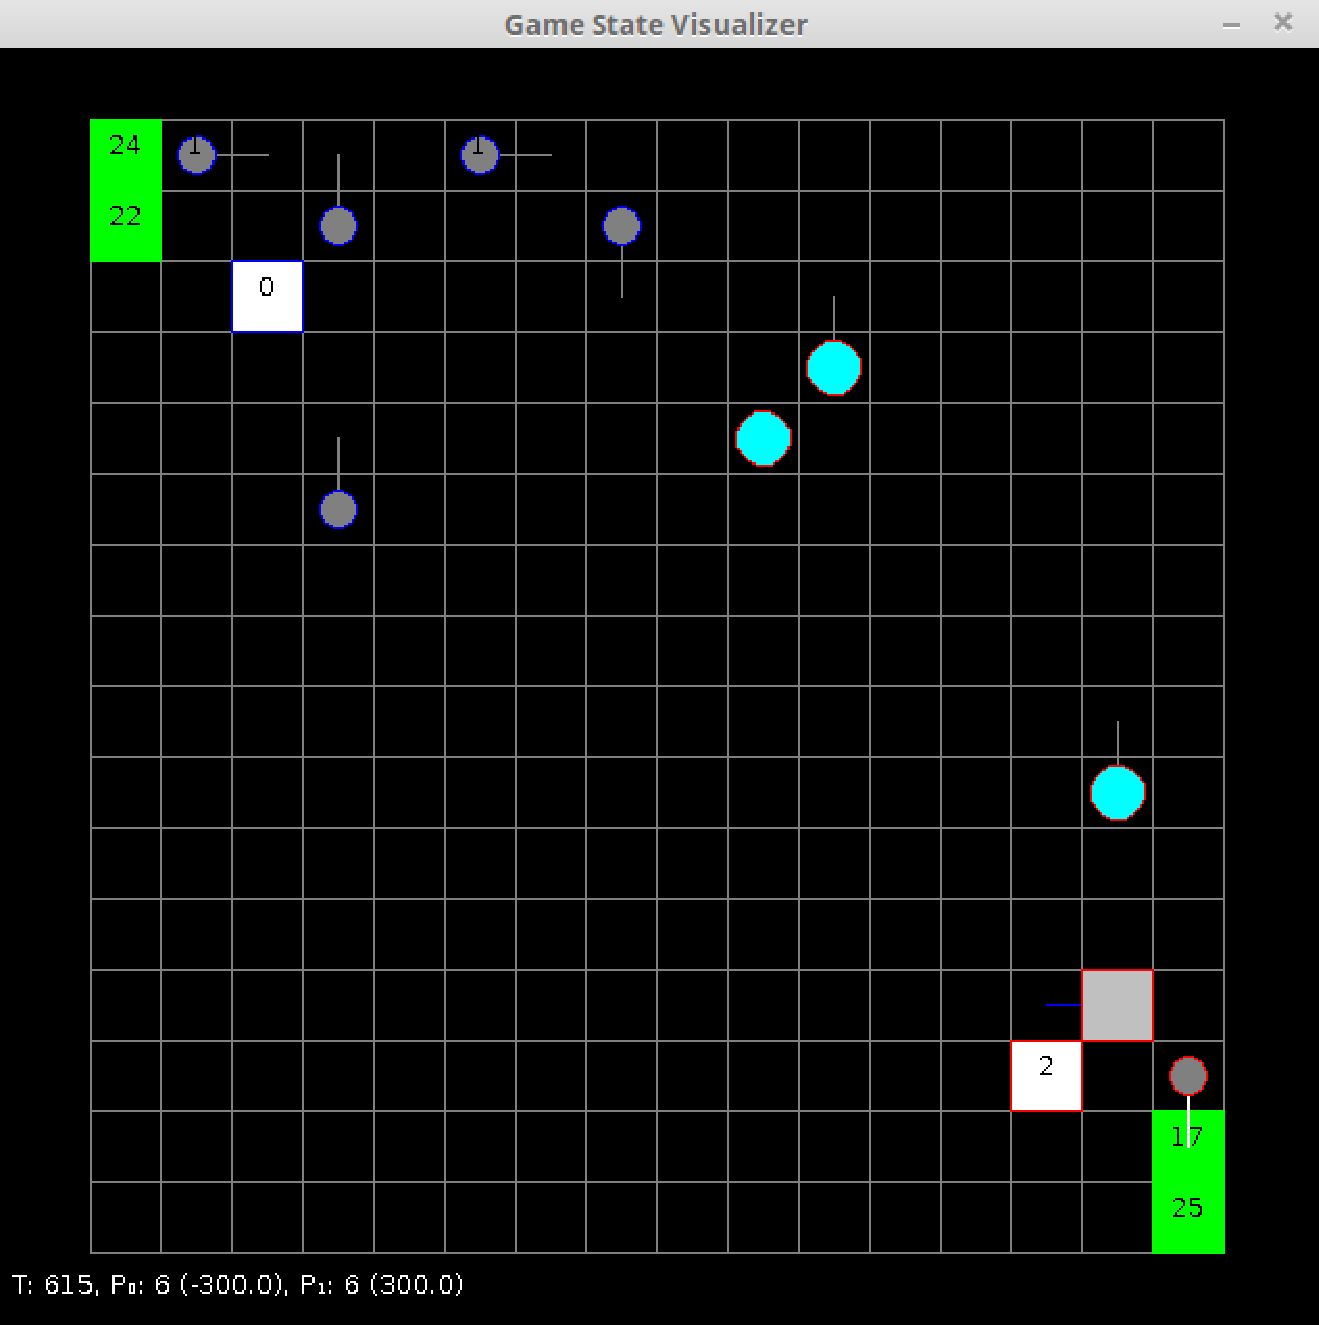
\includegraphics[width=0.6\linewidth]{microRts.pdf}
	\captionof{figure}{Exemplo de tela de um jogo do MicroRTS.}
\end{center}	


%---------------------------------------------------------------
%	Implementação
%---------------------------------------------------------------
\color{NavyBlue}
\section*{\huge Implementa\c{c}\~ao}
\color{Black}

Falar alguma coisa aqui

\vspace{10mm}

\begin{itemize}
	\item Conhecimento de dominio
\end{itemize}


%---------------------------------------------------------------
%	Experimentos e Resultados
%---------------------------------------------------------------
\color{NavyBlue}
\section*{\huge Experimentos e resultados}
\color{Black}

\begin{itemize}
	\item graficozinhos
\end{itemize}


\vspace{13mm}



%---------------------------------------------------------------
% 	Conclusão
%---------------------------------------------------------------
\vspace{-12mm}
\color{NavyBlue}
\section*{\huge Conclus\~ao}
\color{Black}

We have shown empirically that our approach yields not only superior accuracy results but also substantially faster recognition times for all used domains in evaluating against Ram{\'{\i}}rez and Geffner's approach~\cite{RamirezG_IJCAI2009}.

%\begin{itemize}[leftmargin=2em]\itemadjust
%	\item This work addresses the gap in existing norm identification approaches, which assume that violations do not occur, or that when they occur a violation signal is always generated
%	\item We consider two types of evidence:
%	\begin{itemize}
%		%\item Behaviour that is not necessarily always compliant
%                \item Observed traces of other agents, assumed to be generated by plans
%		\item Violation signals, which may be emitted following norm violation
%	\end{itemize}
%	\item An agent using our approach generates norm-compliant behaviour at least $70\%$ in the presence of a large number of norms
%\end{itemize}

%---------------------------------------------------------------
%	Referencias
%---------------------------------------------------------------
\vspace{-9mm}
\large
\color{NavyBlue}
\color{Black}
\raggedright
\bibliographystyle{plain}
\bibliography{poster}

\end{multicols}
%---------------------------------------------------------------
%	Agradecimentos?
%---------------------------------------------------------------
\vspace{-0.5cm}
\hrulefill
\normalsize
\vspace{-1cm}
\section*{Agradecimentos}
\vspace{-1cm}
This research was carried out in cooperation with HP Brazil using incentives of the Brazilian Informatics Law (\# 8.2.48 of 1991).

%----------------------------------------------------------------------------------------
\end{document}